\chapter{Introduzione all'MP3} \label{chap:introduzione_mp3}
	
	\mylettrine{A}{bbiamo} visto, nei capitoli precedenti, che il metodo di campionamento della PCM aveva come obiettivo quello di riprodurre, il più fedelmente possibile, l'onda caratteristica di un segnale audio esterno. Tuttavia questo approccio racchiude in sé un'assunzione implicita, ovvero che sia necessario disporre dell'onda caratteristica per poter riprodurre correttamente un segnale audio. Quest'assunzione nasce sostanzialmente da una scarsa conoscenza della percezione del suono da parte dell'orecchio e del cervello umano.
	
	\section{Codifica percettiva} \label{sec:codifica_percettiva}
		Il problema di fondo è che l'orecchio ed il cervello umano sono  ``strumenti'' imperfetti, che non captano il suono in maniera perfetta e assoluta per come è, ma lo interpretano secondo una serie di fattori. Un esempio è rappresentato dalla soglia assoluta di udibilità umana (in Figure \ref{fig:ath}). È stato dimostrato, inoltre, che raddoppiare l'ampiezza di un segnale audio non corrisponde ad un raddoppiamento dell'effettivo volume percepito. In generale, esistono molti aspetti del suono che l'orecchio ed il cervello umano semplicemente trascurano, accentuando alcune proprietà dei suoni esterni anziché percepire tutto in modo assoluto.\\
		\\
		Come già accennato, la disciplina che si occupa dello studio della percezione del suono prende il nome di \textit{psicoacustica} ed assume un ruolo chiave nella tecnologia MP3.\\
		L'idea di base dell'MP3 è la seguente: se alcune caratteristiche del suono non vengono comunque percepite dall'uomo, perché sprecare spazio inutilmente cercando di riprodurre tutta l'onda caratteristica? Sarebbe molto più intelligente cercare di memorizzare e riprodurre soltanto quelle parti del suono che effettivamente verrano percepite.\\
		Infatti quello che fa l'MP3 è proprio di selezionare le caratteristiche più rilevanti di un certo suono ed assegnargli una maggiore priorità, in modo da riprodurle più fedelmente a scapito di caratteristiche meno rilevanti o superflue. Si potrebbe dire che, mentre la PCM tenta di catturare un segnale audio ``per come è'', l'MP3 tenta di catturarlo ``per come suona''.\\
		\\
		Risulta allora necessario definire cosa è rilevante per l'orecchio umano e cosa non lo è: queste informazioni costituiscono il cosiddetto \textbf{modello psicoacustico}, che definisce quanto e quali parti del suono sono rilevanti.\\
		Prima di entrare nel dettaglio del modello psicoacustico, è necessario definire due concetti chiave: \textit{ridondanza} e \textit{irrilevanza}, che suddividono in due categorie distinte tutte quelle informazioni del suono considerate non necessarie per l'uomo, o comunque eliminabili senza perdere troppo in termini di qualità audio.\\
		Abbiamo già parlato di \textbf{ridondanza} quando abbiamo visto il metodo PCM ed abbiamo parlato del limite di Nyquist: nella qualità CD (frequenza di campionamento di 44.1 \textit{kHz}) tutte le frequenze maggiori di 22.05 \textit{kHz} vengono automaticamente considerate ridondanti, e quindi scartate. Si potrebbe aumentare la sampling frequency, per catturare più alte frequenze, ma il limite in questione non verrebbe eliminato, ma soltanto spostato più in alto. In altre parole, la ridondanza è un concetto onnipresente nel mondo digitale.\\
		L'\textbf{irrilevanza}, invece, è un concetto molto più complesso, che descrive tutte quelle caratteristiche di un'onda sonora che sono prive di senso in termini di percezione umana. Tutte queste caratteristiche, irrilevanti per l'uomo, verranno descritte in un opportuno modello psicoacustico e quindi eliminate (o ridotte di dimensioni) dal file audio finale, diminuendo le dimensioni di quest'ultimo, senza tuttavia influenzarne troppo la qualità, in quanto le informazioni scartate verrebbero comunque ignorate dal cervello umano.
		
	\section{Effetto di mascheramento} \label{sec:effetto_mascheramento}
		
		Il modello psicoacustico utilizzato nella codifica MP3 è basato su un'importante fenomeno, caratteristico dell'orecchio umano, detto \textit{mascheramento} (o \textit{masking} in inglese). Prima di definire cos'è il mascheramento, ricordiamo di seguito il \textit{principio di sovrapposizione} per onde sonore:
		\begin{center}
			\textit{In un punto dello spazio in cui giungono due o più suoni simultanei, il suono risultante è dato dalla somma (algebrica) dei due (o più) suoni incidenti.}
		\end{center}
		Quindi sappiamo che quando due (o più) suoni giungono al nostro orecchio contemporaneamente, quello che noi percepiamo di fatto è la sovrapposizione di questi due (o più) suoni. Questo principio può essere formulato anche al contrario, affermando che ogni suono percepito può essere visto come somma (algebrica) di due o più suoni.\\
		Il nostro cervello e orecchio sono in grado di eseguire, ogni volta che percepiscono un suono esterno, un'analisi spettrografica su di esso, per cercare di ricavarne i suoni generatori. È sempre possibile, per il nostro orecchio, ricavare e distinguere le componenti di un suono composto? La risposta è no, in quanto l'orecchio umano è adattivo e, a seconda della situazione, percepisce stessi suoni in modo diverso. Generalmente, l'orecchio riesce a ricavare le componenti dei suoni che percepisce, distinguendone le varie frequenze, ad eccezione dei seguenti quattro casi:
		\begin{itemize}
			\item quando due suoni simultanei hanno altezze molto simili (\textit{battimenti});
			\item quando uno dei due suoni è molto più forte dell'altro (\textit{mascheramento simultaneo});
			\item quando un suono molto forte precede di poco un suono più debole (\textit{mascheramento temporale in avanti});
			\item quando un suono molto forte segue di poco un suono più debole (\textit{mascheramento temporale all'indietro}).
		\end{itemize}
		Quindi l'effetto di \textbf{mascheramento} è appunto quando la somma di più componenti sonore fa scomparire una delle componenti (mascheramento simultaneo e temporale) o produce un suono totalmente nuovo (battimenti).\\
		\\
		Il \textbf{mascheramento simultaneo} (o \textit{mascheramento a dominio di frequenza}) si ha quando percepiamo un suono predominante assieme ad uno più debole. Un classico esempio è quando proviamo a parlare mentre passa un treno vicino, o c'è un altro rumore forte di sottofondo: il rumore del treno è predominante e verrà percepito più chiaramente, mentre la voce, più debole, verrà percepita con più difficoltà. Più formalmente, si è dimostrato che i suoni percepiti dall'orecchio umano sono suddivisi in 24 \textit{bande critiche}: se più frequenze della stessa banda critica arrivano all'orecchio, quest'ultimo non sarà in grado di distinguere le frequenze originali o comunque verrà percepita soltanto la componente dominante. In Figura \ref{fig:masking_threshold} possiamo vedere come un suono più forte modifichi la soglia di udibilità, rendendo muti suoni prima percepibili. Quando si verifica il mascheramento simultaneo, la soglia di udibilità prende il nome di \textit{soglia di mascheramento} (o \textit{masking threshold} in inglese).\\
		Il \textbf{mascheramento temporale} (o \textit{mascheramento a dominio di tempo}) invece si ha quando un suono predominante precede o segue, in un breve lasso di tempo, un suono più debole. La soglia di tempo necessaria affinché si verifichi il mascheramento temporale è circa 50 \textit{ms} per il mascheramento all'indietro e dai 50 ai 300 \textit{ms} per il mascheramento in avanti \cite{raissi} (si veda la Figura \ref{fig:time_mask}). Possiamo immaginarci il mascheramento temporale pensando ad un ambiente silenzioso in cui improvvisamente si battono le mani: inizialmente il suono delle mani verrà percepito come più forte. Analogamente, se subito prima del battito di mani venisse sparato un colpo di pistola, il battito di mani stesso apparirebbe più attenuato.\\
		
		\begin{figure}[h!]
			\centering
				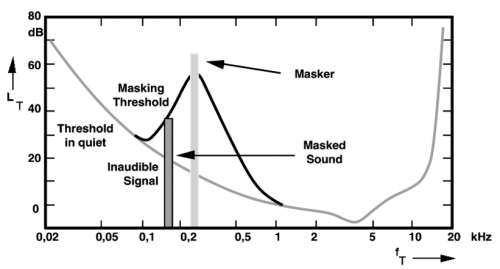
\includegraphics[scale=0.7]{masking_threshold.png}
			\caption{Soglia di mascheramento.}
			\label{fig:masking_threshold}
		\end{figure}
		
		\begin{figure}[h!]
			\centering
				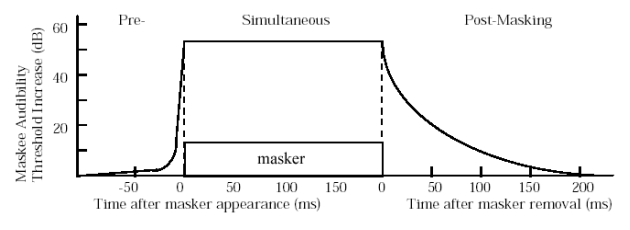
\includegraphics[scale=1]{time_mask.png}
			\caption{Mascheramento temporale.}
			\label{fig:time_mask}
		\end{figure}
		
		L'effetto di mascheramento può essere visto come un'imperfezione dell'orecchio umano, tuttavia rappresenta il punto di forza dell'MP3 e della codifica percettiva: se in un certo lasso di tempo alcune parti del suono vengono percepite con più difficoltà rispetto ad altre, allora possiamo pensare di assegnare più bit per l'informazione del suono predominante e meno per le parti nascoste dal mascheramento. In questo modo l'errore (o distorsione) relativo alle parti mascherate verrà comunque percepito poco, senza degradare più di tanto la qualità complessiva.
		
		